\documentclass[a4paper,twoside]{article}
\usepackage[T1]{fontenc}
\usepackage[bahasa]{babel}
\usepackage{graphicx}
\usepackage{graphics}
\usepackage{float}
\usepackage[cm]{fullpage}
\pagestyle{myheadings}
\usepackage{etoolbox}
\usepackage{setspace} 
\usepackage{lipsum} 
\setlength{\headsep}{30pt}
\usepackage[inner=2cm,outer=2.5cm,top=2.5cm,bottom=2cm]{geometry} %margin
% \pagestyle{empty}

\makeatletter
\renewcommand{\@maketitle} {\begin{center} {\LARGE \textbf{ \textsc{\@title}} \par} \bigskip {\large \textbf{\textsc{\@author}} }\end{center} }
\renewcommand{\thispagestyle}[1]{}
\markright{\textbf{\textsc{AIF184001/AIF184002 \textemdash Rencana Kerja Skripsi \textemdash Sem. Ganjil 2019/2020}}}

\newcommand{\HRule}{\rule{\linewidth}{0.4mm}}
\renewcommand{\baselinestretch}{1}
\setlength{\parindent}{0 pt}
\setlength{\parskip}{6 pt}

\onehalfspacing
 
\begin{document}

\title{\@judultopik}
\author{\nama \textendash \@npm} 

%tulis nama dan NPM anda di sini:
\newcommand{\nama}{Chris Eldon}
\newcommand{\@npm}{2016730073}
\newcommand{\@judultopik}{Privacy Preserving Data Mining dengan Metode Randomization} % Judul/topik anda
\newcommand{\jumpemb}{1} % Jumlah pembimbing, 1 atau 2
\newcommand{\tanggal}{27/08/2019}

% Dokumen hasil template ini harus dicetak bolak-balik !!!!

\maketitle

\pagenumbering{arabic}

\section{Deskripsi}
Dengan semakin banyaknya penambangan data yang dilakukan dan data-data yang digunakan juga semakin banyak, semakin banyak juga privasi-privasi di dalam data tersebut yang tersebar kepada pihak yang melakukan penambangan data. Data-data privasi yang sensitif sangat berpotensi bocor kepada pihak yang tidak bertanggung jawab dan disalahgunakan. Oleh karena itu perlu adanya suatu cara untuk mencegah kebocoran privasi pada proses penambangan data, menjaga privasi pada data-data tersebut. Istilah untuk hal tersebut adalah \textit{Privacy Preserving Data Mining}.

Salah satu cara untuk melakukan \textit{Privacy Preserving Data Mining} adalah dengan memodifikasi data yang ada sebelum diberikan kepada pihak lain. Ada macam-macam teknik dan algoritma yang bertujuan memodifikasi data untuk \textit{Privacy Preserving Data Mining} yang bisa dibagi menjadi dua jenis yaitu \textit{Perturbation Approach} dan \textit{Anonymization Approach}. \textit{Perturbation Approach} adalah pendekatan untuk \textit{Privacy Preserving Data Mining} dengan cara mengacaukan data yang ada, tetapi hasil data yang dikacaukan masih tetap bisa ditambang. \textit{Perturbation Approach} bisa dibagi menjadi dua jenis yaitu \textit{Value-based Perturbation Techniques} dan \textit{Multi-Dimensional Perturbation}.

\textit{Value-based Perturbation Techniques} adalah teknik yang bekerja dengan cara menyisipkan \textit{random noise} pada data. Sedangkan terdapat dua jenis teknik {Multi-Dimensional Perturbation} yaitu \textit{Data mining Task-based Perturbation} dan \textit{Dimension Reduction-based Perturbation}. \textit{Data mining Task-based Perturbation} adalah teknik yang bekerja dengan cara memodifikasi data sehingga properti yang bertahan pada data yang telah dimodifikasi spesifik hanya properti yang digunakan oleh suatu teknik penambangan data tertentu.

\begin{figure}
	\centering
	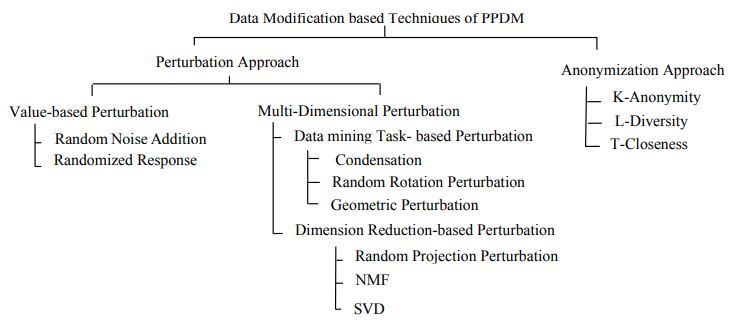
\includegraphics[scale=0.785]{ppdm}
	\caption{Berbagai macam teknik memodifikasi data untuk \textit{Privacy Preserving Data Mining}}
	\label{fig:ppdm}
\end{figure}

Dari berbagai macam teknik memodifikasi data untuk \textit{Privacy Preserving Data Mining} yang dapat dilihat pada Gambar \ref{fig:ppdm}, terdapat empat teknik yang menggunakan metode \textit{Randomization} yaitu \textit{Random Noise Addition}, \textit{Randomized Response}, \textit{Random Rotation Perturbation}, dan \textit{Random Projection Perturbation}.

Pada skripsi ini, akan dibuat sebuah perangkat lunak yang dapat memproses data-data yang akan ditambang menjadi data-data yang telah dimodifikasi dengan metode \textit{Randomization} sehingga tidak mengandung privasi, tetapi masih dapat ditambang.

Dari berbagai macam teknik dengan metode \textit{Randomization} yang ada, dipilih dua buah teknik yaitu \textit{Random Noise Addition} dan \textit{Random Rotation Perturbation} untuk diimplementasikan pada perangkat lunak.

\section{Rumusan Masalah}
\begin{itemize}
	\item Bagaimana cara kerja dari teknik \textit{Random Noise Addition} dan \textit{Random Rotation Perturbation} untuk \textit{Privacy Preserving Data Mining}?
	\item Bagaimana implementasi dari teknik \textit{Random Noise Addition} dan \textit{Random Rotation Perturbation} pada perangkat lunak?
	\item Bagaimana perbandingan antara hasil dari teknik \textit{Random Noise Addition} dan \textit{Random Rotation Perturbation}?
\end{itemize}

\section{Tujuan}
\begin{itemize}
	\item Mempelajari cara kerja dari teknik \textit{Random Noise Addition} dan \textit{Random Rotation Perturbation} untuk \textit{Privacy Preserving Data Mining}
	\item Mengimplementasikan teknik \textit{Random Noise Addition} dan \textit{Random Rotation Perturbation} pada perangkat lunak
	\item Melakukan analisis dan pengujian untuk membandingkan dan mengukur hasil dari teknik \textit{Random Noise Addition} dan \textit{Random Rotation Perturbation}
\end{itemize}

\section{Deskripsi Perangkat Lunak}
Perangkat lunak akhir yang akan dibuat memiliki fitur minimal sebagai berikut:
\begin{itemize}
	\item Pengguna dapat memasukkan data mentah yang akan ditambang (input)
	\item Pengguna dapat memilih teknik mana yang ingin digunakan antara teknik \textit{Random Noise Addition} atau \textit{Random Rotation Perturbation}
	\item Pengguna dapat mengatur berbagai pengaturan seperti parameter untuk teknik \textit{Random Noise Addition} maupun \textit{Random Rotation Perturbation}
	\item Perangkat lunak dapat memodifikasi data mentah yang dimasukkan dengan menggunakan teknik \textit{Random Noise Addition} dan \textit{Random Rotation Perturbation}
	\item Pengguna dapat memperoleh data yang telah diproses dengan teknik \textit{Random Noise Addition} atau \textit{Random Rotation Perturbation} (output)
\end{itemize}

\section{Detail Pengerjaan Skripsi}
Bagian-bagian pekerjaan skripsi ini adalah sebagai berikut :
	\begin{enumerate}
		\item Mempelajari dasar-dasar privasi data
		\item Mempelajari teknik \textit{Random Noise Addition} dan \textit{Random Rotation Perturbation} untuk \textit{Privacy Preserving Data Mining}
		\item Mempelajari teknik penambangan data yang akan digunakan
		\item Melakukan analisis terhadap teknik \textit{Random Noise Addition} dan \textit{Random Rotation Perturbation} serta bagaimana penerapannya dengan teknik penambangan data yang akan digunakan
		\item Melakukan perancangan perangkat lunak yang mengimplementasikan teknik \textit{Random Noise Addition} dan \textit{Random Rotation Perturbation}
		\item Membangun perangkat lunak yang mengimplementasikan teknik \textit{Random Noise Addition} dan \textit{Random Rotation Perturbation}
		\item Menguji perangkat lunak secara fungsional dan eksperimental dengan menggunakan \textit{real} data
		\item Menerapkan teknik penambangan data terhadap data yang telah diproses untuk menganalisis hasil dari teknik \textit{Random Noise Addition} dan \textit{Random Rotation Perturbation}
		\item Melakukan analisis dan pengujian untuk membandingkan dan mengukur hasil dari teknik \textit{Random Noise Addition} dan \textit{Random Rotation Perturbation}
		\item Menulis dokumen skripsi
	\end{enumerate}

\section{Rencana Kerja}
Rincian capaian yang direncanakan di Skripsi 1 adalah sebagai berikut:
\begin{enumerate}
	\item Mempelajari dasar-dasar privasi data
	\item Mempelajari teknik \textit{Random Noise Addition} dan \textit{Random Rotation Perturbation} untuk \textit{Privacy Preserving Data Mining}
	\item Mempelajari teknik penambangan data yang akan digunakan
	\item Melakukan analisis terhadap teknik \textit{Random Noise Addition} dan \textit{Random Rotation Perturbation} serta bagaimana penerapannya dengan teknik penambangan data yang akan digunakan
	\item Menulis dokumen skripsi bab 1, 2, dan 3
\end{enumerate}

Sedangkan yang akan diselesaikan di Skripsi 2 adalah sebagai berikut:
\begin{enumerate}
	\item Melakukan perancangan perangkat lunak yang mengimplementasikan teknik \textit{Random Noise Addition} dan \textit{Random Rotation Perturbation}
	\item Membangun perangkat lunak yang mengimplementasikan teknik \textit{Random Noise Addition} dan \textit{Random Rotation Perturbation}
	\item Menguji perangkat lunak secara fungsional dan eksperimental dengan menggunakan \textit{real} data
	\item Menerapkan teknik penambangan data terhadap data yang telah diproses untuk menganalisis hasil dari teknik \textit{Random Noise Addition} dan \textit{Random Rotation Perturbation}
	\item Melakukan analisis dan pengujian untuk membandingkan dan mengukur hasil dari teknik \textit{Random Noise Addition} dan \textit{Random Rotation Perturbation}
	\item Menulis dokumen skripsi bab 4, 5, dan 6
\end{enumerate}

\vspace{1cm}
\centering Bandung, \tanggal\\
\vspace{2cm} \nama \\ 
\vspace{1cm}

Menyetujui, \\
\ifdefstring{\jumpemb}{2}{
\vspace{1.5cm}
\begin{centering} Menyetujui,\\ \end{centering} \vspace{0.75cm}
\begin{minipage}[b]{0.45\linewidth}
% \centering Bandung, \makebox[0.5cm]{\hrulefill}/\makebox[0.5cm]{\hrulefill}/2013 \\
\vspace{2cm} Nama: \makebox[3cm]{\hrulefill}\\ Pembimbing Utama
\end{minipage} \hspace{0.5cm}
\begin{minipage}[b]{0.45\linewidth}
% \centering Bandung, \makebox[0.5cm]{\hrulefill}/\makebox[0.5cm]{\hrulefill}/2013\\
\vspace{2cm} Nama: \makebox[3cm]{\hrulefill}\\ Pembimbing Pendamping
\end{minipage}
\vspace{0.5cm}
}{
% \centering Bandung, \makebox[0.5cm]{\hrulefill}/\makebox[0.5cm]{\hrulefill}/2013\\
\vspace{2cm} Nama: \makebox[3cm]{\hrulefill}\\ Pembimbing Tunggal
}
\end{document}

